In this section, we describe the measurement model for a single-pixel
time-of-flight lidar sensor under diffuse, pulsed laser illumination. 
\subsection{Measurement Model}
Consider a laser which emits a pulse at time $t = 0$ with time-varying intensity
$g(t)$ uniformly illuminating some 3D scene. We parameterize the geometry of the
scene as a height map $z(x, y)$.
Neglecting albedo and falloff effects, an ideal detector counting photon events
from a location $(x,y)$ in the time interval $(n\Delta t, (n+1) \Delta t)$ would record

\begin{equation}
  \lambda_{x,y}[n] = \int_{n\Delta t}^{(n+1) \Delta t} (f * g)\paren*{t - 2z(x,y)/c} dt \label{single_loc_spad} 
\end{equation}  

where $c$ is the speed of light, and $f$ is a function that models the temporal uncertainty in the
detector. Single-photon avalanche diodes (SPADs) are highly sensitive
photodetectors which are able to record single photon events with high temporal
precision \cite{Stuff}. Since the detection of each photon can be described with
a Bernoulli random variable,
the total number of accumulated photons in this time interval follows a Poisson
distribution according to

\begin{equation}
  h[n] \sim \mathcal{P}\paren*{\sum_{x,y}\alpha_{x,y}\eta \lambda_{x,y}[n] + b} \label{global_hints}
\end{equation}

where $\alpha_{x,y} = r_{x,y}/z(x,y)^2$ captures the attenuation of the
photon counts due to the reflectance $r(x,y)$ of the scene and due to the
inverse square falloff $1/z(x,y)^2$.
In addition, $\eta$ is the detection probability of a photon
triggering a SPAD event, and $b = \eta a + d$ is the average number of background detections resulting
from ambient photons $a$
and erroneous ``dark count'' events $d$ resulting from noise within the SPAD.
\newpage
\begin{table*}[htbp]
  \begin{center}
    \begin{tabularx}{\linewidth}{*{2}{X}}
      \includegraphics[width=\textwidth/2-5pt]{sections/figures/spad_example/rgb.png} &
      \includegraphics[width=\textwidth/2-5pt]{sections/figures/spad_example/rawdepth.png} \\
      \includegraphics[width=\textwidth/2-5pt]{sections/figures/spad_example/depth_hist.png} &
      \includegraphics[width=\textwidth/2-5pt]{sections/figures/spad_example/spad_hist.png} \\
    \end{tabularx}
  \end{center}
  \caption{Sample Image. Top Left is the RGB image. Top Right is ground truth
    depth. Bottom Left is Raw ground truth depth histogram. Bottom Right is
    simulated SPAD measurements. Notice how closer depths are magnified and far
    depths are attenuated.}
\end{table*}

\subsection{Monocular depth estimation with global depth hints}
Given a single RGB image $I(x,y)$ and a vector of photon arrivals $h[n]$
described by equation \ref{global_hints}, we seek to
reconstruct the ground truth depth map $z(x,y)$.
Our method has two parts. First, we initialize our estimate of the depth map from the single RGB
image via a monocular depth estimator described below. Second, we refine this depth map using
the captured measurements $h[n]$ via a process we call Differentiable Histogram
Matching (DHM).
Differentiable histogram matching is a tool for post-processing the image to
match the depth map to the statistics we capture from the SPAD.

\paragraph{Initialization via CNN}
Convoluational Neural Networks have become increasingly capable of leveraging
monocular depth cues to produce accurate estimates of depth
from only a single image. We therefore choose to initialize our depth map
estimate $\hat z^{(0)}(x,y)$ using
a CNN. However, any depth estimator reliant on only a single
view will be unable to resolve the inherent scale ambiguity in the scene resulting
from the tradeoff between size of and distance to an object. The next step,
differentiable histogram matching, will resolve this ambiguity using the depth
information present in the SPAD histogram.

\paragraph{Differentiable Histogram Matching}
Given our initial depth map estimate, our goal is now to refine that depth map
so that it agrees with the information provided by the SPAD histogram.
Figure showing just the differentiable histogram matching part of the model.
At a high level, we perform local optimization over the pixels of the depth map
to make it consistent with the observed measurements $h[n]$.
Given per-pixel depth, we can simulate SPAD histogram formation using equation
\ref{global_hints}, where we approximate $\lambda_{x,y}[n]$ using kernel density
estimation \cite{something} as:
\begin{equation}
  \hat \lambda^{(i)}_{x,y}[n] = \frac{1}{\sigma\sqrt{2 \pi}}\exp\paren*{-\frac{1}{2\sigma^2}(n - \hat z^{(i)}(x,y))} \label{KDE}
\end{equation}
where $\hat z^{(i)}(x, y)$ is our estimate of the depth at pixel $(x,y)$ at
iteration $i$.

Once we have $\lambda^{(i)}$, we compute $\hat h[n]$ according to the rest of
the SPAD histogram formation model (neglecting the Poisson sampling) as follows
\begin{equation}
  \hat h[n] = \sum_{x,y}\alpha_{x,y}\eta \lambda_{x,y}[n] + b. \label{diff_forward}
\end{equation}
Finally, given two histograms, we can compute the Wasserstein Distance between
them. As described in \ref{Cuturi et. al.}, the Wasserstein Distance or ``earth
mover's distance'' measures the distance between two probability distributions
by calculating the minimum cost of moving the mass required to turn the first
distribution into the second. It is particularly desirable
because unlike the KL divergence or the simple RMSE, the Wasserstein Distance scales with
separation as well as magnitude (see figure). Although the computation of the
Wasserstein Distance requires solving a linear program, there is a regularized
version known as the dual-Sinkhorn Distance
which can be computed via Sinkhorn-Knopp Iterations in a fast and differentiable manner.
We refer the reader to \ref{Cuturi et. al.} for details, but provide the
optimization problem here.

Given histograms $h, \hat h$ in $\Delta^n$ and a cost matrix $C$ in $\R^{n \times
  n}$, the dual-Sinkhorn Divergence is found by solving
the optimization problem
\begin{equation}
    \begin{aligned}
    &\text{minimize} && \langle W, C \rangle  - \frac{1}{\lambda}h(W) \\
    &\text{subject to} && W^Th = \bm{1} \\
    &                  && W\hat h = \bm{1} \\
    &                  && W \succeq 0 \\
  \end{aligned}
\end{equation}
where $W \in \Delta^{n \times n}$ is the optimization variable, $\bm{1}$ denotes the
vector of all ones, $h(\cdot)$ is the entropy of a probability distribution, and
$\langle \cdot, \cdot \rangle$ denotes the inner product of two matrices.
\begin{itemize}
\item Pseudocode for sinkhorn iterations?
  \item Not sure what figure to use...
\end{itemize}
\newpage
\begin{figure}
  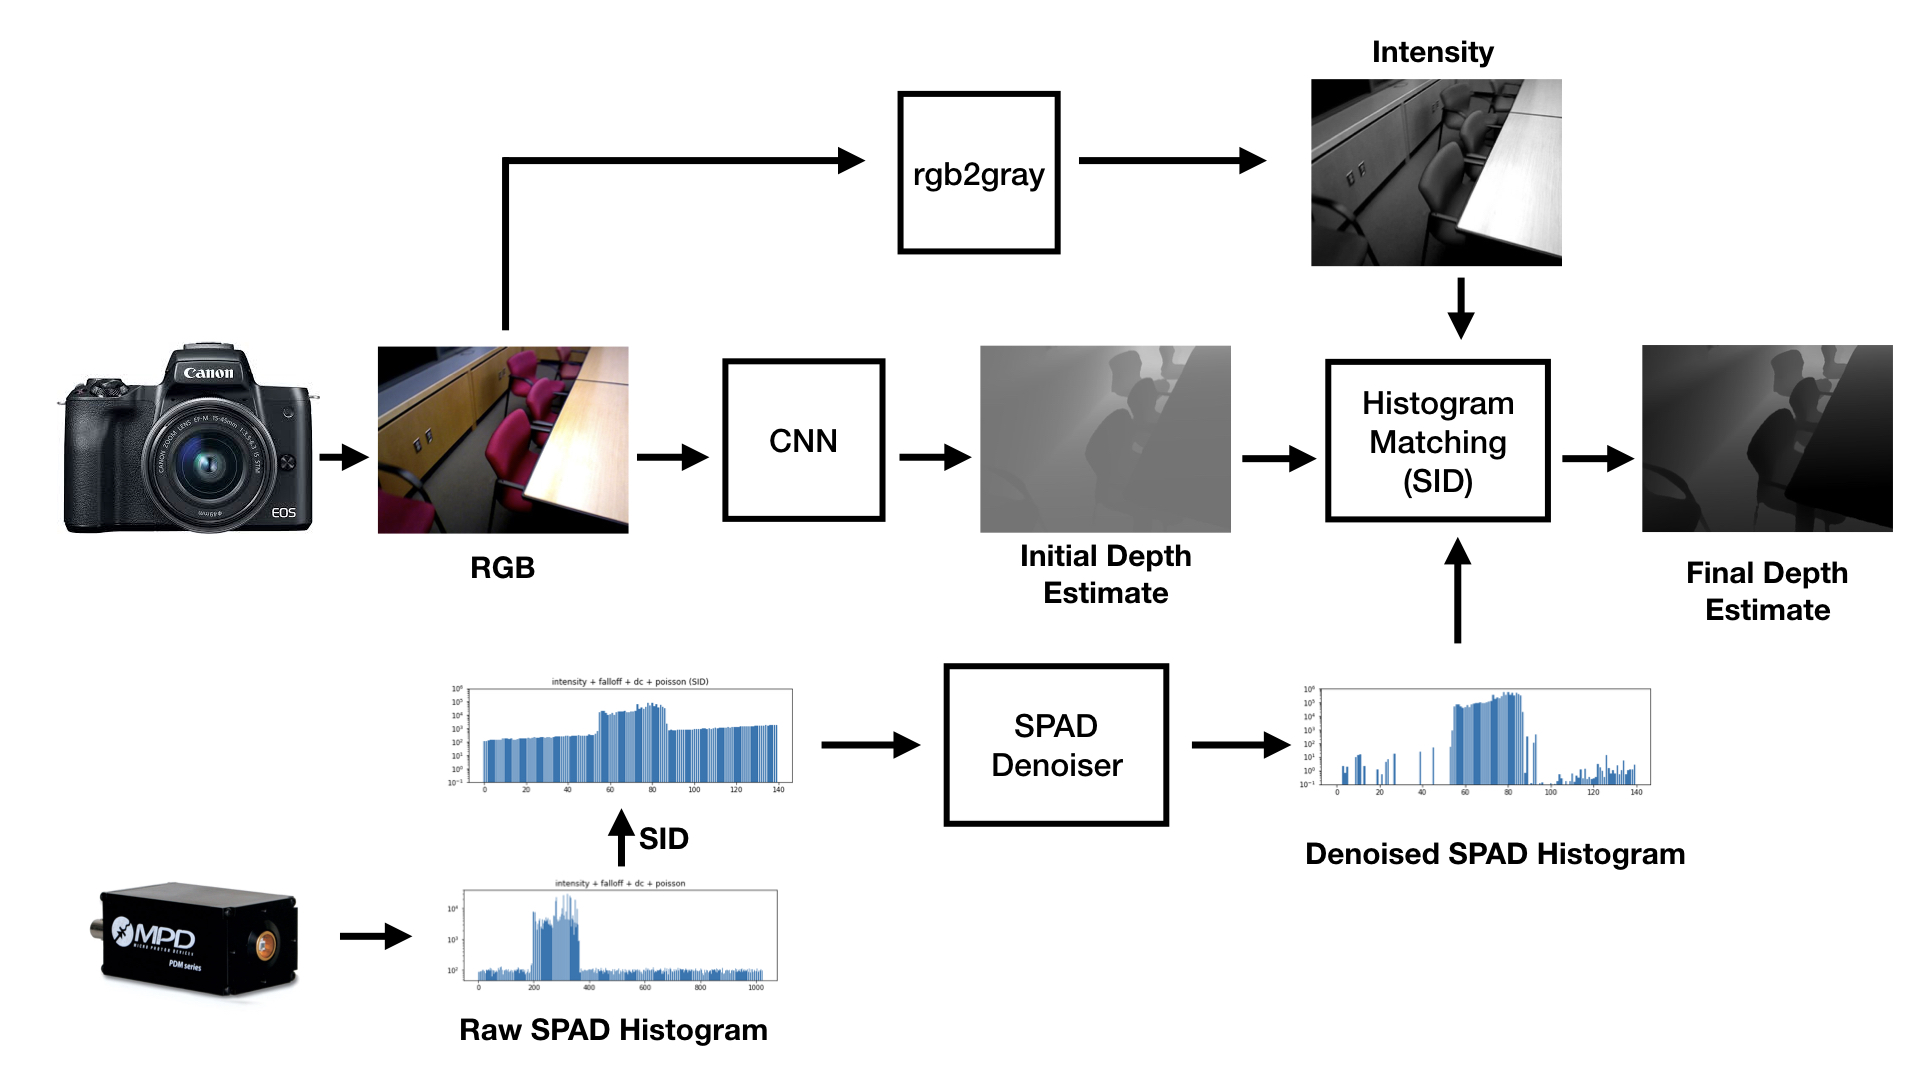
\includegraphics[width=\textwidth/2]{sections/figures/full_pipeline/full_pipeline.png}
  \caption{\textbf{Overview of the full pipeline} We use a CNN to get an initial
  per-pixel depth estimate. We then perform gradient descent to optimize that
  estimate using the SPAD forward model and the dual-Sinkhorn distance.}
\end{figure}


\subsection{Implementation Details}
For the Monocular Depth Estimator, we use a pretrained version of the
the Deep Ordinal Regression Network (DORN) \cite{}. We use the implementation of
the Sinkhorn Iteration (for calculating the dual-Sinkhorn distance)
from \ref{Cuturi et. al.} We update the depth map using gradient descent.
Everything is implemented in PyTorch.
We run the model on a NVIDIA Titan X GPU, where it takes approximately 5 seconds
to fully process a single RGB-SPAD data pair.
Table with hyperparameters (defer to supplementary info?)
\begin{itemize}
\item Kernel Density Estimation (sigma)
\item Sinkhorn Iterations (maximum number, epsilon tolerance)
\item Gradient Descent (learning rate, epsilon tolerance, max iterations)
\item Simulation hyperparameters ($\eta, b$)
\end{itemize}


